% В этом файле следует писать текст работы, разбивая его на
% разделы (section), подразделы (section) и, если нужно,
% главы (chapter).

% Предварительно следует указать необходимую информацию
% в файле SETUP.tex

%% В этот файл не предполагается вносить изменения

% В этом файле следует указать информацию о себе
% и выполняемой работе.

\documentclass [fontsize=14pt, paper=a4, pagesize, DIV=calc]%
{scrartcl}
% ВНИМАНИЕ! Для использования глав поменять
% scrartcl на scrreprt

% Здесь ничего не менять
\usepackage [T2A] {fontenc}   % Кириллица в PDF файле
\usepackage [utf8] {inputenc} % Кодировка текста: utf-8
\usepackage [russian] {babel} % Переносы, лигатуры

%%%%%%%%%%%%%%%%%%%%%%%%%%%%%%%%%%%%%%%%%%%%%%%%%%%%%%%%%%%%%%%%%%%%%%%%
% Создание макроса управления элементами, специфичными
% для вида работы (курс., бак., маг.)
% Здесь ничего не менять:
\usepackage{ifthen}
\newcounter{worktype}
\newcommand{\typeOfWork}[1]
{
	\setcounter{worktype}{#1}
}

% ВНИМАНИЕ!
% Укажите тип работы: 0 - курсовая, 1 - бак., 2 - маг.,
% 3 - бакалаврская с главами.
\typeOfWork{1}
% Считается, что курсовая и бак. бьются на разделы (section) и
% подразделы (subsection), а маг. — на главы (chapter), разделы и
%  подразделы. Если хочется,
% чтобы бак. была с главами (например, если она большая),
% надо выбрать опцию 3.

% Если при выборе 2 или 3 вы забудете поменять класс
% документа на scrreprt (см. выше, в самом начале),
% то получите ошибку:
% ./aux/appearance.tex:52: Package scrbase Error: unknown option ` chapterprefix=

%%%%%%%%%%%%%%%%%%%%%%%%%%%%%%%%%%%%%%%%%%%%%%%%%%%%%%%%%%%%%%%%%%%%%%%%
% Информация об авторе и работе для титульной страницы

\usepackage {titling}

% Имя автора в именительном падеже (для маг.)
\newcommand {\me}{%
И.\,И.~Иванов%
}

% Имя автора в родительном падеже (для курсовой и бак.)
\newcommand {\byme}{%
О.\,Е.~Филиппской%
}

% Любимый научный руководитель
\newcommand{\supervisor}%
{асс. каф. ИВЭ А.\,М. Пеленицын}

% идентифицируем пол (только для курсовой и бак.)
\newcommand{\bystudent}{
Студентки % Для курсовой: с большой буквы
}

% Год публикации
\date{2016}

% Название работы
\title{Генерация экземпляров классов типов\\на на основе экземпляров производных классов\\в языке Haskell}

% Кафедра
%
\newboolean{needchair}
\setboolean{needchair}{true} % на ФИИТ не пишется (false), на ПМИ есть (true)

\newcommand {\thechair} {%
Кафедра информатики и вычислительного эксперимента%
}

\newcommand {\direction} {%
Направление подготовки\\
Прикладная математика и информатика%
}% Прикладная математика и информатика

%%%%%%%%%%%%%%%%%%%%%%%%%%%%%%%%%%%%%%%%%%%%%%%%%%%%%%%%%%%%%%%%%%%%%%%%
% Другие настраиваемые элементы текста

% Листинги с исходным кодом программ: укажите язык программирования
\usepackage{listings}
\lstset{
    language=[ISO]C++,%  Язык указать здесь
    basicstyle=\small\ttfamily,
    breaklines=true,%
    deletekeywords={Monad,Functor,return,liftM,ap},
    morekeywords={where, instance, data, class, of},
    showstringspaces=false%
    inputencoding=utf8x%
    literate={\{}{\textcolor{black}{\{}}1
             {\}}{\textcolor{black}{\}}}1
             {[}{\textcolor{black}{[}}1     
             {]}{\textcolor{black}{]}}1
}
% полный список языков, поддерживаемых данным пакетом, есть,
% например, здесь (стр. 13):
% ftp://ftp.tex.ac.uk/tex-archive/macros/latex/contrib/listings/listings.pdf

% Нумерация списков: можно при необходимести
% изменять вид нумерации (например, добавлять правую скобку).
% По умолчанию буду списки вида:
% 1.
% 2.
% Изменять вид нумерации можно в начале нумерации:
% \begin{enumerate}[1)] (В квадратных скобках указан желаемый вид)
\usepackage[shortlabels]{enumitem}
                    \setlist[enumerate, 1]{1.}

% Гиперссылки: настройте внешний вид ссылок
\usepackage%
[pdftex,unicode,pdfborder={0 0 0},draft=false,%backref=page,
    hidelinks, % убрать, если хочется видеть ссылки: это
               % удобно в PDF файле, но не должно появиться на печати
    bookmarks=true,bookmarksnumbered=false,bookmarksopen=false]%
{hyperref}


\usepackage {amsmath}      % Больше математики
\usepackage {amssymb}
\usepackage {textcase}     % Преобразование к верхнему регистру
\usepackage {indentfirst}  % Красная строка первого абзаца в разделе

\usepackage {fancyvrb}     % Листинги: определяем своё окружение Verb
\DefineVerbatimEnvironment% с уменьшенным шрифтом
	{Verb}{Verbatim}
	{fontsize=\small}

% Вставка рисунков
\usepackage {graphicx}

% Общее оформление
% ----------------------------------------------------------------
% Настройка внешнего вида

%%% Шрифты

% если закомментировать всё — консервативная гарнитура Computer Modern
\usepackage{paratype} % профессиональные свободные шрифты
%\usepackage {droid}  % неплохие свободные шрифты от Google
%\usepackage{mathptmx}
%\usepackage {mmasym}
%\usepackage {psfonts}
%\usepackage{lmodern}
%var1: lh additions for bold concrete fonts
%\usepackage{lh-t2axccr}
%var2: the package below could be covered with fd-files
%\usepackage{lh-t2accr}
%\usepackage {pscyr}

% Геометрия текста

\usepackage{setspace}       % Межстрочный интервал
\onehalfspacing

\newlength\MyIndent
\setlength\MyIndent{1.25cm}
\setlength{\parindent}{\MyIndent} % Абзацный отступ
\frenchspacing            % Отключение лишних отступов после точек
\KOMAoptions{%
    DIV=calc,         % Пересчёт геометрии
    numbers=endperiod % точки после номеров разделов
}

                            % Консервативный вариант:
%\usepackage                % ручное задание геометрии
%[%                         % (не рекомендуется в проф. типографии)
%  margin = 2.5cm,
  %includefoot,
  %footskip = 1cm
%] %
%  {geometry}

%%% Заголовки

\ifthenelse{{\value{worktype} > 1}}{%
  \KOMAoptions{%
      headings=normal,   % размеры заголовков поменьше стандартных
      chapterprefix=true,% Печатать слово Глава
      appendixprefix=true% Печатать слово Приложение
  }
}{% Печатать слово Приложение даже если нет глав
  \newcommand*{\appendixmore}{%
%    \renewcommand*{\sectionformat}{%
%       \appendixname~\thesection\autodot\enskip}
    \renewcommand*{\sectionmarkformat}{%
      \appendixname~\thesection\autodot\enskip}
  }
}

% шрифт для оформления глав и названия содержания
\newcommand{\SuperFont}{\Large\sffamily\bfseries}

% Заголовок главы
\ifthenelse{\value{worktype} > 1}{%
\renewcommand{\SuperFont}{\Large\normalfont\sffamily}
\newcommand{\CentSuperFont}{\centering\SuperFont}
\usepackage{fncychap}
\ChNameVar{\SuperFont}
\ChNumVar{\CentSuperFont}
\ChTitleVar{\CentSuperFont}
\ChNameUpperCase
\ChTitleUpperCase
}

% Заголовок (под)раздела с абзацного отступа
\addtokomafont{sectioning}{\hspace{\MyIndent}}

\renewcommand*{\captionformat}{~---~}
\renewcommand*{\figureformat}{Рисунок~\thefigure}

% Плавающие листинги
\usepackage{float}
\floatstyle{ruled}
\floatname{ListingEnv}{Листинг}
\newfloat{ListingEnv}{htbp}{lol}[section]

% точка после номера листинга
\makeatletter
\renewcommand\floatc@ruled[2]{{\@fs@cfont #1.} #2\par}
\makeatother


%%% Оглавление
\usepackage{tocloft}

% шрифт и положение заголовка
\ifthenelse{\value{worktype} > 1}{%
\renewcommand{\cfttoctitlefont}{\hfil\SuperFont\MakeUppercase}
}{
\renewcommand{\cfttoctitlefont}{\hfil\SuperFont}
}

% слово Глава
\usepackage{calc}
\ifthenelse{\value{worktype} > 1}{%
\renewcommand{\cftchappresnum}{Глава }
\addtolength{\cftchapnumwidth}{\widthof{Глава }}
}

% Очищаем оформление названий старших элементов в оглавлении
\ifthenelse{\value{worktype} > 1}{%
\renewcommand{\cftchapfont}{}
\renewcommand{\cftchappagefont}{}
}{
\renewcommand{\cftsecfont}{}
\renewcommand{\cftsecpagefont}{}
}

% Точки после верхних элементов оглавления
\renewcommand{\cftsecdotsep}{\cftdotsep}
%\newcommand{\cftchapdotsep}{\cftdotsep}

\ifthenelse{\value{worktype} > 1}{%
    \renewcommand{\cftchapaftersnum}{.}
}{}
\renewcommand{\cftsecaftersnum}{.}
\renewcommand{\cftsubsecaftersnum}{.}
\renewcommand{\cftsubsubsecaftersnum}{.}

%%% Списки (enumitem)

\usepackage {enumitem}      % Списки с настройкой отступов
\setlist %
{ %
  leftmargin = \parindent, itemsep=.5ex, topsep=.4ex
} %

% По ГОСТу нумерация должны быть буквами: а, б...
%\makeatletter
%    \AddEnumerateCounter{\asbuk}{\@asbuk}{м)}
%\makeatother
%\renewcommand{\labelenumi}{\asbuk{enumi})}
%\renewcommand{\labelenumii}{\arabic{enumii})}

%%% Таблицы: выбрать более подходящие

\usepackage{booktabs} % считаются наиболее профессионально выполненными
%\usepackage{ltablex}
%\newcolumntype {L} {>{---}l}

%%% Библиография

\usepackage{csquotes}        % Оформление списка литературы
\usepackage[T1]{fontenc}
\usepackage[
  backend=biber,
  hyperref=auto,
  sorting=none, % сортировка в порядке встречаемости ссылок
  language=auto,
  citestyle=gost-numeric,
  bibstyle=gost-numeric
]{biblatex}
\addbibresource{biblio.bib} % Файл с лит.источниками

% Настройка величины отступа в списке
\ifthenelse{\value{worktype} < 2}{%
\defbibenvironment{bibliography}
  {\list
     {\printtext[labelnumberwidth]{%
    \printfield{prefixnumber}%
    \printfield{labelnumber}}}
     {\setlength{\labelwidth}{\labelnumberwidth}%
      \setlength{\leftmargin}{\labelwidth}%
      \setlength{\labelsep}{\dimexpr\MyIndent-\labelwidth\relax}% <----- default is \biblabelsep
      \addtolength{\leftmargin}{\labelsep}%
      \setlength{\itemsep}{\bibitemsep}%
      \setlength{\parsep}{\bibparsep}}%
      \renewcommand*{\makelabel}[1]{\hss##1}}
  {\endlist}
  {\item}
}{}

% ----------------------------------------------------------------
% Настройка переносов и разрывов страниц

\binoppenalty = 10000      % Запрет переносов строк в формулах
\relpenalty = 10000        %

\sloppy                    % Не выходить за границы бокса
%\tolerance = 400          % или более точно
\clubpenalty = 10000       % Запрет разрывов страниц после первой
\widowpenalty = 10000      % и перед предпоследней строкой абзаца

% ----------------------------


% Стили для окружений типа Определение, Теорема...
% Оформление теорем (ntheorem)

\usepackage [thmmarks, amsmath] {ntheorem}
\theorempreskipamount 0.6cm

\theoremstyle {plain} %
\theoremheaderfont {\normalfont \bfseries} %
\theorembodyfont {\slshape} %
\theoremsymbol {\ensuremath {_\Box}} %
\theoremseparator {:} %
\newtheorem {mystatement} {Утверждение} [section] %
\newtheorem {mylemma} {Лемма} [section] %
\newtheorem {mycorollary} {Следствие} [section] %

\theoremstyle {nonumberplain} %
\theoremseparator {.} %
\theoremsymbol {\ensuremath {_\diamondsuit}} %
\newtheorem {mydefinition} {Определение} %

\theoremstyle {plain} %
\theoremheaderfont {\normalfont \bfseries} 
\theorembodyfont {\normalfont} 
%\theoremsymbol {\ensuremath {_\Box}} %
\theoremseparator {.} %
\newtheorem {mytask} {Задача} [section]%
\renewcommand{\themytask}{\arabic{mytask}}%
\newtheorem {myremark} {Замечание} %

\theoremheaderfont {\scshape} %
\theorembodyfont {\upshape} %
\theoremstyle {nonumberplain} %
\theoremseparator {} %
\theoremsymbol {\rule {1ex} {1ex}} %
\newtheorem {myproof} {Доказательство} %

\theorembodyfont {\upshape} %
%\theoremindent 0.5cm
\theoremstyle {nonumberbreak} \theoremseparator {\\} %
\theoremsymbol {\ensuremath {\ast}} %
\newtheorem {myexample} {Пример} %
\newtheorem {myexamples} {Примеры} %

\theoremheaderfont {\itshape} %
\theorembodyfont {\upshape} %
\theoremstyle {nonumberplain} %
\theoremseparator {:} %
\theoremsymbol {\ensuremath {_\triangle}} %
\theoremstyle {nonumberbreak} %
\newtheorem {myremarks} {Замечания} %


% Титульный лист
% Макросы настройки титульной страницы
% В этот файл не предполагается вносить изменения

%\usepackage {showframe}

% Вертикальные отступы на титульной странице
\newcommand{\vgap}{\vspace{16pt}}

% Помещение города и даты в нижний колонтитул
\usepackage{scrlayer}
\DeclareNewLayer[
  foot,
  foreground,
  contents={%
    \raisebox{\dp\strutbox}[\layerheight][0pt]{%
      \parbox[b]{\layerwidth}{\centering Ростов-на-Дону\\ \thedate%
       \\\mbox{}
       }}%
  }
]{titlepage.foot.fg}
\DeclareNewPageStyleByLayers{titlepage}{titlepage.foot.fg}


\AtBeginDocument %
{ %
  %
  \begin{titlepage}
  %
    \thispagestyle{titlepage}

    {\centering
    %
    \MakeTextUppercase {МИНИСТЕРСТВО ОБРАЗОВАНИЯ И НАУКИ РФ}

    \vgap

    Федеральное государственное автономное образовательное\\
    учреждение высшего образования\\
    \MakeTextUppercase {Южный федеральный университет}

    \vgap

	Институт математики, механики и компьютерных наук
    имени~И.\,И.\,Воровича

    \vgap

    \direction

    \ifthenelse{\boolean{needchair}}{
    \vgap

    \thechair}{}

    \vspace* {\fill}

    \ifthenelse{\value{worktype} = 2}{%
    \me

    \vgap}{}

    {\usefont{T2A}{PTSansCaption-TLF}{m}{n}
    \MakeTextUppercase{\thetitle}}

    \ifthenelse{\value{worktype} = 2}{%
     \vgap

    Выпускная квалификационная работа\\
    на степень магистра}{}
    \ifthenelse{\value{worktype} = 0}{
     \vgap

    Курсовая работа
    }{}%
    \ifthenelse{\value{worktype} = 1 \OR \value{worktype} = 3}{
     \vgap

    Выпускная квалификационная работа\\
    на степень бакалавра
    }{}%

    \vspace {\fill}

    \begin{flushright}
    \ifthenelse{\value{worktype} = 0 \OR 
                \value{worktype} = 1 \OR
                \value{worktype} = 3}{
      \bystudent \ifthenelse{\value{worktype} = 0}{3}{4}\ курса\\
      \byme
    }{}

    \vgap

    Научный руководитель:\\
    \supervisor\\
    \ifthenelse{\value{worktype} = 2}{%
    Рецензент:\\
    ученая степень, ученое звание, должность
    И. О. Фамилия
    }{}
	\end{flushright}
    \ifthenelse{\value{worktype} = 0}{
    \vspace{\fill}
            \begin{flushleft}
              \begin{tabular}{cc}
                \underline{\hspace{4cm}}&\underline{\hspace{5cm}}\\
                {\small оценка (рейтинг)} & {\small  подпись руководителя}\\
              \end{tabular}
            \end{flushleft}
    }{}
  	\vspace {\fill}
  %Ростов-на-Дону

    %\thedate

  }\end{titlepage}
  %
  %
  \tableofcontents
  %
  \clearpage
} %



% Команды для использования в тексте работы


% макросы для начала введения и заключения
\newcommand{\Intro}{\addsec{Введение}}
\ifthenelse{\value{worktype} > 1}{%
    \renewcommand{\Intro}{\addchap{Введение}}%
}

\newcommand{\Conc}{\addsec{Заключение}}
\ifthenelse{\value{worktype} > 1}{%
    \renewcommand{\Conc}{\addchap{Заключение}}%
}

% Правильные значки для нестрогих неравенств и пустого множества
\renewcommand {\le} {\leqslant}
\renewcommand {\ge} {\geqslant}
\renewcommand {\emptyset} {\varnothing}

% N ажурное: натуральные числа
\newcommand {\N} {\ensuremath{\mathbb N}}

% значок С++ — используйте команду \cpp
\newcommand{\cpp}{%
C\nolinebreak\hspace{-.05em}%
\raisebox{.2ex}{+}\nolinebreak\hspace{-.10em}%
\raisebox{.2ex}{+}%
}

% Неразрывный дефис, который допускает перенос внутри слов,
% типа жёлто-синий: нужно писать жёлто"/синий.
\makeatletter
    \defineshorthand[russian]{"/}{\mbox{-}\bbl@allowhyphens}
\makeatother


\endinput

% Конец файла

\hyphenation{Monad Applicative Functor Control Data}
    \tikzstyle{every node}=[shape=rectangle, color=black, rounded corners,%
    text=black, anchor=west]
    \tikzstyle{selected}=[shape=rectangle, rounded corners,%
    top color=gray,%
    bottom color=gray, text=white]
    \tikzstyle{optional}=[dashed,fill=gray!50]

\begin{document}

\Intro
\section*{Цель работы}
\section*{Постановка задачи}

\chapter{Предварительные сведения}

\chapter{Алгоритм выведения типов}
\section{Основные понятия}
Для начала введём основные термины, которые будут использоваться при описании алгоритма выведения типов.
\begin{description}
	\item[Компонент.] Компонентами являются встроенные функции. <Добавить также изображение компонента>
	\item[Функция.] Если не указано иное, функцией будем называть определённую пользователем функцию.
	\item[Вызывающий компонент (caller).] Компонент, предназначающийся для использования определённой пользователем функции.
	\item[Связь (connection).]
	\item[Вход (connection point).] Вход компонента соответствует одному аргументу функции. На вход можно подать значение (одно из возможных значений типа, который назначен данному входу) либо другой компонент. Компонент может не иметь входов, если это: 
	\begin{enumerate}[1)]
		\item аргумент определяемой пользователем функции;
		\item вызывающий компонент (caller) пользовательской функции без аргументов.
	\end{enumerate} 
	\item[Контекст.] description
	\item[Инферер (inferer).] description
	\item[Алиас (alias).] description
\end{description}
 
\chapter{Проблемы и их решения}

\chapter{Детали реализации}

\chapter{Кодогенерация}
\section{Постановка задачи кодогенерации}
Для программы на визуальном языке сгенерировать соответствующий ей код на языке Haskell. Полученный код должен компилироваться с помощью GHC. Затем корневая функция должна вычислиться, а её результат~--- передаться в основную программу.
\section{План решения}
Решение поставленной задачи состоит из следующих шагов.
\begin{enumerate}[1.]
	\item На стороне Haskell:
		\begin{enumerate}[1)]
			\item создавать GHC-контекст, в который помещать определения функций из стандартных модулей (включая базовый модуль Prelude);
			\item генерировать код на основе данных, полученных из основной программы;
			\item компилировать полученный код и помещать в созданный на шаге 1.1 контекст новые определения;
			\item вызывать требуемую функцию и её результат передавать в основную программу;
			\item если выполнение или компиляция завершились с ошибкой, т.е. произошёл выброс исключения, сообщить об этом основной программе.
		\end{enumerate}
	\item На стороне C++:
		\begin{enumerate}[1)]
			\item передать стороне Haskell данные для генерации кода;
			\item получить результат вычисления требуемой функции.
		\end{enumerate}
\end{enumerate}
\section{Программные средства}
Для решения данной задачи было решено использовать следующие средства языка Haskell.

	\subsection{Template Haskell (TH)} Template Haskell~--- стандартный фреймворк, предоставляющий средства для типобезопасного метапрограммирования на языке Haskell, обрабатываемые на этапе компиляции компилятором GHC. [ссылка на хаскель вики]  TH позволяет писать мета-программы на языке Haskell, результатом выполнения которых являются другие программы на языке Haskell. Данный фреймворк применяется для кодогенерации во времени выполнения а также для создания доменно-специфичных языков. Для решения нашей задачи нам потребуется возможность сгенерировать синтаксическое дерево (представляемое специальными типами данных) и получить его строковое представление (т.е. в виде программного кода на языке Haskell) с помощью функций структурной печати (англ. \textit{pretty-printing}).
	
	\subsubsection{Основные используемые типы данных} Для кодогенерации нам понадобятся следующие типы данных: \lstinline!data Exp! и \
	\lstinline!data Dec!. Первый из них представляет собой тип данных, отвечающим \textit{выражению} на языке Haskell, т.е. этим типом данных описываются переменные, литералы, применения функций, условные выражения и т.д. (см. табл. \ref{expconstr}). Второй описывает \textit{определения} на языке Haskell, например, функции, определения новых типов данных, классов типов, синонимов типов и др. (см. табл. \ref{decconstr}).
	
	\subsubsection{Возможные проблемы} Среди программистов на языке Haskell использование TH считается небезопасным [ссылка на ugly but necessary]. Этому есть причины. Например, с помощью TH можно сгенерировать такой код, который не будет компилироваться (не пройдёт проверку типов) [ссылка на what's so bad about TH]. Тем не менее, мы будем предполагать, что алгоритм выведения типов нашего визуального языка работает корректно, а потому сгенерированный таким образом код будет рабочим.
	
\begin{table}[h]
	\begin{center}
		\begin{tabular}{ll}
			{\lstinline!VarE Name!} & имя переменной \\
			{\lstinline!ConE Name!} & имя конструктора типа данных \\
			{\lstinline!LitE Lit!} & литерал (числовой или символьный) \\
			{\lstinline!AppE Exp Exp!} & применение функции \\
			{\lstinline!InfixE (Maybe Exp) Exp (Maybe Exp)!} & бинарная операция, возможно, \\ & частично применённая \\
			{\lstinline!LamE [Pat] Exp!} & лямбда-выражение \\
			{\lstinline!TupE [Exp]!} & кортеж \\
			{\lstinline!CondE Exp Exp Exp!} & условное выражение \\
			{\lstinline!ListE [Exp]!} & список \\
		\end{tabular}
	\end{center}
\caption{Некоторые конструкторы типа данных Exp}
\label{expconstr}
\end{table}

\begin{table}[h]
\begin{center}
	\begin{tabular}{ll}
		{\lstinline!FunD Name [Clause]!} & определение функции \\
										 & {\lstinline!func x y = ...!} \\
		{\lstinline!SigD Name Type!} & прототип (сигнатура) функции \\
									 & {\lstinline!func :: a -> a -> a!}
	\end{tabular}
\end{center}
\caption{Некоторые конструкторы типа данных Dec}
\label{decconstr}
\end{table}
	% Библиотека для метапрограммирования на языке Haskell. Предоставляет возможность генерировать код на языке Haskell с помощью специальных типов данных, затем возвращать его строковое представление с помощью функций структурной печати (\textit{pretty-printing}). Не гарантирует, что сгенерированный таким образом код пройдёт проверку системы типов. Однако будем предполагать, что такую гарантию нам даёт наш собственный алгоритм выведения типов.
	\subsection{GHC API~--- программный интерфейс компилятора}\label{ghcapisec} Функционал GHC может быть использован не только для компиляции программ на языке Haskell. Важным примером использования может послужить анализ и, возможно, преобразование кода на языке Haskell. Другим примером является динамическая загрузка кода, как	в GHCi [4]. Для этих целей функционал GHC доступен через библиотеку GHC API.
	
	Рассмотрим некоторые модули этой библиотеки, функционал которых применялся в данной работе.
	\begin{description}
		\item[InteractiveEval.] Предоставляет функции для манипуляции выражениями языка Haskell, в том числе и для их исполнения. Работа с выражениями происходит в специально создающемся для этого контексте интерактивных вычислений (англ. interactive evaluation context). Этот контекст содержит все определения, которые в него были помещены. В него можно импортировать и определения стандартных модулей.
		\item[DynFlags.] В этом модуле описаны параметры компиляции. Большинство флагов являются динамическими. Это означает, что они могут изменяться от одного процесса компиляции к другому.
		\item[HsImpExp.] Здесь содержатся типы данных и функции, предназначенные для работы с импортом модулей. Модуль в языке Haskell можно подключить различными способами: стандартным образом (т.е. использовать все определения из него), импортируя только конкретные функции, запрещая импортировать некоторые функции и так далее. Функционал модуля HsImpExp позволяет это сделать, например, для интерактивного контекста.
		\item[GHC.] Модуль, посвящённый работе с монадой GHC. Это монада, содержащая весь функционал, необходимый для вызовов функций GHC API. 
	\end{description} 

	Более подробно см. документацию по GHC API [ссылка]. % API компилятора GHC. Для решения поставленной задачи мы воспользуемся такими возможностями этой библиотеки, как создание контекста и привнесение в него определений (которые мы будем генерировать с помощью Template Haskell), а также исполнение функций интерпретатором. 
	\subsection{Foreign Function Interface (FFI)} Это расширение стандарта языка Haskell. Оно позволяет программам на языке Haskell взаимодействовать с программами, написанными на других языках. Таким образом, с помощью этого расширения программы на языке Haskell могут вызывать программы, написанные на других языках, и наоборот: программы на различных языках получают возможность вызывать программы на языке Haskell. В нашем случае мы будем использовать средства взаимодействия с языком C. 
	
	\subsubsection{Соглашение о вызове} Для того, чтобы взаимодействовать с кодом, написанным на другом языке, необходимо знать \textit{соглашение о вызове} (англ. \textit{calling convention}), использующееся реализацией другого языка в текущей архитектуре. С помощью FFI компилятор языка Haskell GHC поддерживает стандартные соглашения о вызове, такие как \lstinline{cdecl}, \lstinline{pascal} и другие. Например, пусть при объявлении функции, предназначенной для другого языка программирования, указано соглашение о вызове \lstinline{cdecl}. Тогда GHC сгенерирует такой код, при исполнении которого параметры будут расположены в памяти и в регистрах таким образом, как того ожидает компилятор языка C (или любой другой компилятор, использующий то же соглашение о вызове). А именно, аргументы функций передаются справа налево; очистку стека производит вызывающая программа.
	
	Соглашение о вызове зависит от типов параметров. Только некоторые типы данных языка Haskell могут быть напрямую использованы для функций, предназначенных для других языков, потому что эти типы данных отвечают базовым типам данных низкоуровневых языков программирования. Рассмотрим некоторые типы данных, которые будут нами позднее использованы.
	
	\subsubsection{Основные используемые типы данных} Значение типа \lstinline{Ptr a} представляет собой указатель на объект или массив объектов, который может быть маршалирован (англ. \textit{marshalled}) в значения языка Haskell типа \lstinline{a} (или наоборот, из массива значений языка Haskell в массив значений другого языка). Тип данных \lstinline{a}, как правило, является экземпляром класса \lstinline{Storable}, который предоставляет операции маршалинга (англ. \textit{marshalling}). Однако это не существенно: пользователь может реализовать собственные операции доступа к указателю.
	
	Также нам понадобится тип данных \lstinline{CWString}. Он является синонимом типа данных \lstinline{Ptr CWchar} и представляет собой указатель на массив символов в кодировке Unicode в языке C, завершающийся пустым символом (т.е. \lstinline{wchar_t*} в языке C).
	
	\textit{Устойчивый указатель} (англ. \textit{stable pointer})~--- это ссылка на выражение языка Haskell, значение которого сборщиком мусора гарантировано не будет ни удалено (т.~е. память, выделенная под него, не будет освобождена), ни перемещено в другую область памяти. Таким образом, устойчивые указатели могут быть переданы в код на другом языке программирования, который будет обращаться с ними как с ссылками на значения языка Haskell, закреплённые в памяти (аналогом такой конструкции можно считать закреплённый указатель (англ. \textit{pinned pointer}) в языке C\#). Таким образом, мы сможем создать контекст, представленный монадой \textit{Ghc}, создать устойчивый указатель на него, а затем использовать его в языке C. Со стороны языка C мы будем манипулировать им как указателем типа~\lstinline{void*}.   % Библиотека языка Haskell, которая позволяет создавать функции на языке Haskell, предназначенные для исполнения их на другом языке программирования (в данном случае C/C++). Позволяет работать с некоторыми типами данных языков C/C++, в том числе позволяет создавать указатели, что нам пригодится для работы с контекстом.

\section{Решение и детали реализации решения}
	\subsection{Создание GHC-контекста}
		Для начала создадим GHC-контекст, куда поместим определения из стандартных модулей. Для этого определим функцию \lstinline!mkModuleImport!, которая принимает строку, а возвращает \lstinline!InteractiveImport!~--- тип данных, описывающий подключение модуля (см. листинг \ref{mkmod}). Предусмотрим ситуацию конфликта имён функций, то есть когда в разных модулях имеются определения функций с одинаковыми именами. Добавим для этого возможность не импортировать определённые функции из модуля, если они не потребуются. Итак, если строка-параметр состоит только из имени модуля, тогда создаём простой импорт модуля (соответствует объявлению \lstinline!import ModuleName!) с помощью функции \lstinline!simpleImportDecl!. В противном случае создаём объявление импорта модуля вида \lstinline!import ModuleName hiding (name1, name2, ...)!, то есть в котором указано, объекты с какими именами импортировать не нужно (это могут быть функции, типы данных, классы типов и т. д.).
		
		Непосредственно созданием контекста занимается функция \lstinline!createContext! (см. листинг \ref{crcont}). Эта функция принимает список строк (имена стандартных модулей) и возвращает монаду Ghc (см. гл. \ref{ghcapisec}). Здесь мы устанавливаем флаги для текущей сессии компиляции:
		\begin{enumerate}[1)]
			\item \lstinline!hscTarget!~--- тип кода, который будет являться результатом компиляции, в нашем случае это байткод;
			\item \lstinline!ghcLink!~--- что требуется сделать на этапе компоновки; здесь будем использовать компоновщик, отправляющий код сразу в память, без записи на диск.
		\end{enumerate}
	
		Затем мы подключаем стандартные модули и помещаем все имена из них в созданный контекст с помощью функции \lstinline!getnamesInScope!. Базовый GHC-контекст создан.
		
		\begin{ListingEnv}[h]
		\begin{lstlisting}
mkModuleImport :: String -> InteractiveImport
mkModuleImport mod_info = 
	let info = splitOn " " mod_info
 	in case (length info) of
		1 -> IIDecl $ simpleImportDecl 
			    $ mkModuleName mod_info
		_ -> let simple_import = simpleImportDecl 
			    $ mkModuleName (head info)
			 string_names  = tail info
                         names         = map (noLoc . IEVar . noLoc . mkRdrUnqual .mkVarOcc) string_names
                     in IIDecl 
              $ ImportDecl { 
              ideclSourceSrc = ideclSourceSrc simple_import
            , ideclName      = ideclName simple_import
	    , ideclPkgQual   = ideclPkgQual simple_import
	    , ideclSource    = ideclSource simple_import
	    , ideclSafe      = ideclSafe simple_import
	    , ideclQualified = ideclQualified simple_import
	    , ideclImplicit  = ideclImplicit simple_import
	    , ideclAs        = ideclAs simple_import
	    , ideclHiding    = Just (False, noLoc names) 
	  }
		\end{lstlisting}
		\caption{Реализация функции mkModuleImport} \label{mkmod}
		\end{ListingEnv}
	
		\begin{ListingEnv}[h]
		\begin{lstlisting}
createContext :: [String] -> Ghc [Name]
createContext stmods = do
		dflags <- getSessionDynFlags
		setSessionDynFlags 
			$ dflags { hscTarget = HscInterpreted
			         , ghcLink   = LinkInMemory }
		setContext (map mkModuleImport stmods)
		getNamesInScope
		\end{lstlisting}
		\caption{Реализация функции createContext} \label{crcont}
		\end{ListingEnv}
		
	\subsection{Генерация кода}
		\subsubsection{Определения новых типов данных}
		Нам понадобится промежуточное представление для синтаксического дерева программы. Именно в таком виде сторона Haskell будет получать данные для кодогенерации со стороны C++. Определим тип данных \textit{Expression} (см. листинг \ref{expdata}). У этого типа данных несколько конструкторов:
		\begin{enumerate}[1)]
			\item \lstinline!Param!, описывает параметр функции в её теле;
			\item \lstinline!Literal!, описывает числовой, символьный или логический литералы;
			\item \lstinline!Call!, описывает применение функции (стандартной или определённой пользователем), сюда также относятся конструкторы списка и кортежа;
			\item \lstinline!PartApply!, описывает вызов частично применённой функции.			
		\end{enumerate}
		
		Введём также вспомогательные типы данных: \textit{BinaryOp} для бинарных операций, \textit{UnaryOp} для унарных операций, \textit{HsType} для встроенных типов данных.
		
		\begin{ListingEnv}[h]
		\begin{lstlisting}[language=Haskell]
data Expression = Param String
	        | Literal HsType String
                | Call CallInfo HsType [Expression]
                | PartApply [Expression] Expression
                | Empty
deriving (Read, Show, Eq)	
	
data CallInfo = BuiltIn String | Custom String | Binary BinaryOp | Unary UnaryOp
deriving (Read, Show, Eq)
		\end{lstlisting}
		\caption{Определение типа данных Expression}\label{expdata}
		\end{ListingEnv}
		
		\subsubsection{Непосредственно кодогенерация}
	\subsection{Взаимодействие между кодами на языках C++ и Haskell}
\section{Пример работы кодогенератора}
Для демонстрации работы кодогенератора поступим следующим образом. Изобразим в IDE визуального языка программу. Для неё вручную напишем соответствующий ей код на языке Haskell, чтобы затем сравнить его с кодом, который даст кодогенератор. После скомпилируем и выполним обе программы и сравним результаты.

Изобразим программу вычисления длины целочисленного списка рекурсивным образом (см. рис. \ref{lengthrec}). Затем напишем код, который соответствует изображённому нами синтаксическому дереву (см. табл. \ref{expectreal}, левая колонка). 

Теперь получим промежуточное представление синтаксического дерева (см. листинг \ref{intermed}). Из промежуточного представления видно, что имеется две функции: основная функция, вычисляющая длину конкретного списка с помощью функции, определённой пользователем, и собственно функция вычисления длины списка, определённая пользователем. Основная функция не имеет аргументов и вложенных функций. Функция вычисления длины целочисленного списка имеет один аргумент (собственно список) и также не имеет вложенных функций. Это полностью отвечает тому, что мы изобразили в IDE.

Получаем код, который создаёт кодогенератор (см. табл. \ref{expectreal}, правая колонка). Видно, что он абсолютно идентичен коду, который был написан вручную: различаются только имена функций и их аргументов, порядок функций в программе.

Наконец, исполним функции с названием \lstinline!root! из обеих колонок табл. \ref{expectreal} и сравним результаты их вычислений. Результаты вычислений представлены в таблице \ref{exprealres}. Вычисление обеих функций дало одинаковый результат.

\begin{figure}[p]
\centering
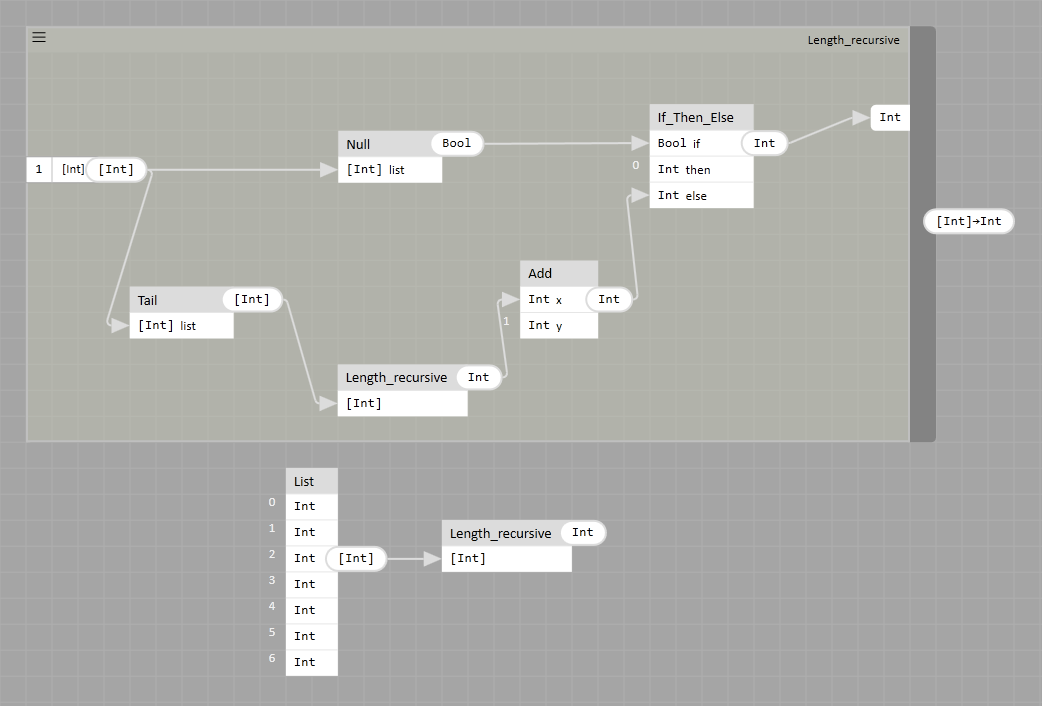
\includegraphics[width=\textwidth]{img/length.PNG}
\caption{Реализация функции, вычисляющей длину списка, и её применение} \label{lengthrec}	
\end{figure}

\begin{ListingEnv}[h]
\begin{lstlisting}
FunctionDef {
    fun_name = "root"
  , args = []
  , result = HsInt
  , body = Call (Custom "function1") (HsInt) 
          [Call (BuiltIn "list") (HsList (HsInt)) 
          [Literal HsInt "0"
         , Literal HsInt "1"
         , Literal HsInt "2"
         , Literal HsInt "3"
         , Literal HsInt "4"
         , Literal HsInt "5"
         , Literal HsInt "6"]]
  , nested_funs = []
 }
 
FunctionDef {
    fun_name = "function1"
  , args = [FunctionArg {
              arg_name = "function1_arg0"
            , arg_type = HsList (HsInt)}]
  , result = HsInt
  , body = Call (BuiltIn "if") (HsInt) 
          [Call (BuiltIn "null") (HsBool) 
          [Param "function1_arg0"]
        , Literal HsInt "0"
        , Call (Binary Add) (HsInt) 
          [Call (Custom "function1") (HsInt) 
          [Call (BuiltIn "tail") (HsList (HsInt)) 
          [Param "function1_arg0"]]
        , Literal HsInt "1"]]
  , nested_funs = []
 }
\end{lstlisting}
\caption{Промежуточное представление программы}\label{intermed}
\end{ListingEnv}

\begin{table}[h]
\centering
\begin{tabular}{|l|l|}
\hline
Код, написанный программистом &
Сгенерированный код \\
\hline
\begin{lstlisting}
length_rec :: [Int] -> Int
length_rec xs = 
 if null xs
  then 0
  else length_rec (tail xs) + 1

root :: Int
root = 
 length_rec [0, 1, 2, 3, 4, 5, 6]
\end{lstlisting} &
\begin{lstlisting}
root :: Int
root = 
 function1 [0, 1, 2, 3, 4, 5, 6]

function1 :: [Int] -> Int
function1 function1_arg0 = 
 if null function1_arg0
  then 0
  else 
   function1 (tail function1_arg0)
     + 1
\end{lstlisting} \\
\hline
\end{tabular}
\caption{Сравнение ожидаемого и сгенерированного кода}\label{expectreal}
\end{table}

\begin{table}[h]
\centering
\begin{tabular}{|l|l|}
\hline
Ожидаемые результаты & Полученные результаты \\
\hline
 & \\
\begin{minipage}{2in}
	\begin{verbatim}
*Main> root
7
	\end{verbatim}
\end{minipage} &
~~~~~~~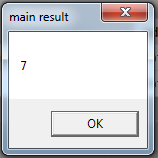
\includegraphics{img/result.PNG} \\
 & \\
\hline
\end{tabular}
\caption{Сравнение результатов вычислений ожидаемой и сгенерированной функции}\label{exprealres}
\end{table}

\chapter{Тестирование}
\section{Тест <<Переприсоединение>>}
Тест <<Переприсоединение>> (англ. \textit{test-reconnect}) был задумал с целью автоматизации проверки того, что состояние инферера каждого компонента остаётся прежним после удаления и восстановления одной из входящих связей.
\section{Тест <<Все ко всем>>}
Тест <<Все ко всем>> (англ. \textit{all-to-all test}) воспроизводит попытки создания всевозможных связей для каждого конкретного примера. Это необходимо для проверки того, что все ошибочные ситуации обрабатываются правильно. К ошибочным ситуациям относятся:
\begin{itemize}
	\item попытка создания связи, которая приводит к циклу в синтаксическом дереве;
	\item попытка создания связи, которая приводит к появлению бесконечного типа;
\end{itemize}


% Печать списка литературы (библиографии)
\printbibliography[%{}
    heading=bibintoc%
    %,title=Библиография % если хочется это слово
]
% Файл со списком литературы: biblio.bib
% Подробно по оформлению библиографии:
% см. документацию к пакету biblatex-gost
% http://ctan.mirrorcatalogs.com/macros/latex/exptl/biblatex-contrib/biblatex-gost/doc/biblatex-gost.pdf
% и огромное количество примеров там же:
% http://mirror.macomnet.net/pub/CTAN/macros/latex/contrib/biblatex-contrib/biblatex-gost/doc/biblatex-gost-examples.pdf

%\appendix
%\ifthenelse{\value{worktype} > 1}{%
  %\addtocontents{toc}{%
      %\protect\renewcommand{\protect\cftchappresnum}{\appendixname\space}%
      %\protect\addtolength{\protect\cftchapnumwidth}{\widthof{\appendixname\space{}} - \widthof{Глава }}%
  %}%
%}{
  %\addtocontents{toc}{%
      %\protect\renewcommand{\protect\cftsecpresnum}{\appendixname\space}%
      %\protect\addtolength{\protect\cftsecnumwidth}{\widthof{\appendixname\space{}}}%
  %}%
%}

%\section{Пример работы программы}

%Здесь длинный листинг с примером работы.

\end{document}
